\documentclass[10pt]{beamer}
\usetheme{Warsaw}

\usepackage[utf8]{inputenc}
\usepackage[francais]{babel}
\usepackage[T1]{fontenc}
\usepackage{amsmath}
\usepackage{amsfonts}
\usepackage{amssymb}
\usepackage{graphicx}

%% Test
\newcommand\boxmath[1]{$\rouge{\boxed{#1}}$}
\usepackage{tcolorbox}

%% Couleurs %%
\usepackage{xcolor}
\definecolor{bleu}{RGB}{14, 68, 175}
\definecolor{bleu3}{RGB}{222, 233, 255 }
\definecolor{orange2}{RGB}{255, 216, 154}
\definecolor{rouge}{RGB}{201, 0, 0}
\definecolor{vert}{RGB}{14, 137, 0}
\definecolor{gris}{RGB}{222,230,230}
\newcommand\rouge[1] {{\color{rouge}{#1}}}
\newcommand\bleu[1] {{\color{bleu}{#1}}}
\newcommand\green[1]{{\color{vert}{#1}}}

\graphicspath{{images/}}
\author{Sami AS}
\title{Résumé MS2}

\begin{document}

\begin{frame}
\titlepage
\end{frame}

\begin{frame}
\tableofcontents
\end{frame}
\section{Mécanique du solide}
\subsection{Les contraintes}
\begin{frame}{Le tenseur de contraintes}
La mécanique des solides diffère de la mécanique rationnelle parce que les solides se \underline{déforment}. Ils vont donc développer des efforts internes, et la notion de \textit{tenseur de contraintes} intervient pour les quantifier.
\begin{block}{Tenseur de contraintes de Cauchy}
\boxmath{T_i ^{(n)} \equiv \tau_{ji} n_j} est l'écriture du tenseur de contraintes. Il s'agit d'un tenseur d'ordre 2, ce qui veut dire que l'élément $T_i^{(n)}$ est un \textbf{vecteur}.
\end{block}
Une contrainte représente un effort interne par unité de surface, et est toujours associée à un plan de coupe, lui défini par une normale extérieure. La contrainte représente alors \textbf{l'action de la partie coupée sur la partie qu'on étudie.}
\end{frame}

\begin{frame}{Remarques et propriétés des tenseurs}


\begin{block}{Propriétés des tenseurs d'ordre 2}
\begin{itemize}
\item $\exists$ directions principales : celles pour lesquelles la composante normale du vecteur de contrainte est maximale. \boxmath{\tan(2\theta) = \frac{2\tau_{xy}}{\sigma_x - \sigma_y}}
\item $\exists$ valeurs principales qui sont la valeur de contrainte normale principale associée à une direction principale. %%\boxmath{\sigma_{1,2} = \frac{\sigma_x + \sigma_y}{2} \pm \sqrt{\left(\frac{\sigma_x - \sigma_y}{2} \right)^2 + \tau_{xy} ^2}}
\item On peut définir le tenseur dans d'autres axes à l'aide de la formule de changement d'axes : \boxmath{T' _{PQ} = \alpha_{Pi} \alpha_{Qj} T_{ij}}.
\end{itemize}
\end{block}
\strut \\
\begin{minipage}{\textwidth}
\begin{columns}[T]
\begin{column}{0.7\textwidth}
\small \underline{Remarque} : on mesure les contraintes grâce au tenseur de Cauchy une fois que le solide a été déformé (suite aux forces de volume, de surface), donc \textbf{à l'équilibre après déformation}. Cependant il arrive souvent qu'on le représente dans l'état initial sans déformation parce qu'on considère des petites déformations.
\end{column}
\begin{column}{0.3\textwidth}
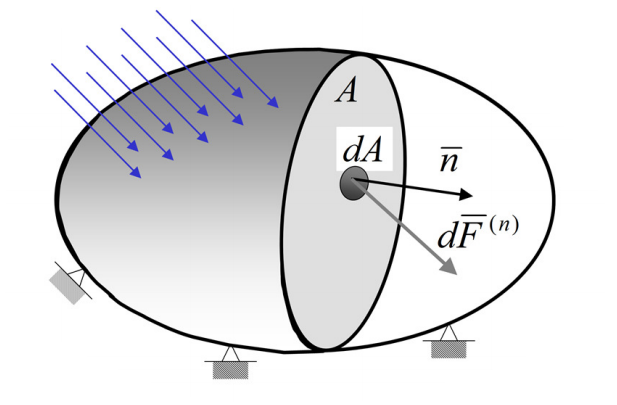
\includegraphics[width=3.5cm]{MS2-1}
\end{column}
\end{columns}
\end{minipage}

\end{frame}
\subsection{Les déformations}
\begin{frame}{Les déformations dans un solide}
\begin{itemize}
\item Déformations naturelles : \textbf{non-linéaires}, ce sont les déformations de Lagrange. On les garde dans un tenseur de déformation : le \textbf{tenseur de déformation de Lagrange} $L_{jk}$.
\item Déformations linéaires : c'est la partie symétrique du gradient de déplacement, qu'on utilise pour des \textbf{petites déformations}. Le tenseur associé aux petites déformations (donc linéaires) est noté $\varepsilon_{ij}$.
\end{itemize}
\begin{block}{Tenseurs de déformations}
\begin{center}
$L_{jk} =\frac{1}{2} (u_{j,i} + u_{i,j} + u_{i,j}u_{i,k}) \qquad \strut$ \boxmath{\varepsilon_{ij} = \frac{1}{2} (u_{j,i} + u_{i,j})}
\end{center}
\end{block}

\end{frame}
\subsection{Les lois de comportement}
\begin{frame}{Lois de comportement}
On lie les déformations et les contraintes à travers les lois de comportement. Pour des déformations linéaires, on utilise les lois de \textbf{Hooke}.
\begin{block}{Lois de Hooke : $\varepsilon_{ij} \leftrightarrow \tau_{ij}$}
\begin{eqnarray}
\varepsilon_{ij} &=& \dfrac{1}{E} \left[(1+\nu) \tau_{ij} - \nu\ \delta_{ij}\ \tau_{kk} \right] \\
\tau_{ij} &=& \dfrac{E}{1+\nu}\left[\varepsilon_{ij} + \dfrac{\nu}{1-2\nu}\ \delta_{ij}\ \varepsilon_{kk} \right]
\end{eqnarray}
\end{block}
\end{frame}
\begin{frame}{Lois fondamentales de la mécanique}
Avec :
\begin{itemize}
\item Forces de volume $f_i$
\item Masse volumique $\rho$
\end{itemize}
On peut écrire les lois suivantes.
\begin{block}{Lois fondamentales}
\begin{itemize}
\item Résultante cinétique : \boxmath{\rho v^\circ _i =  \tau_{ji, \ j} + f_i}. C'est la loi de Newton $\vec{f} = m \vec{a}$, avec les forces de volumes et de surface (c'est la dérivée de $\tau_{ij}$ parce que l'intégrale de surface des forces de surfaces (= les contraintes) est passée en intégrale de volume de la divergence par le théorème de Gauss). On déduit l'équation d'équilibre de translation en statique : \boxmath{f_i + \partial_j \tau_{ij} = 0}. Les forces de volumes équilibre le \textbf{gradient de contraintes}.
\item Moment cinétique : \boxmath{\tau_{ij} = \tau_{ji}}. Le tenseur est donc symétrique.
\end{itemize}
\end{block}
\end{frame}
\subsection{Remarques d'après-TP}
\begin{frame}{Formules utiles}
\begin{block}{Cercle de Mohr : changement d'axes et valeurs principales}
\begin{itemize}
\item Les valeurs principales : $\sigma_{I, II} = \dfrac{\sigma_x + \sigma_y}{2} \pm \sqrt{\left( \dfrac{\sigma_x - \sigma_y}{2}\right)^2 + \tau_{xy} ^2}$
\item Les contraintes lors dans les nouveaux axes :
\begin{center}
$\left\{ \begin{array}{l}

\sigma_u = \dfrac{\sigma_x + \sigma_y}{2} + \dfrac{\sigma_x - \sigma_y}{2} \ \cos(2\theta) + \tau_{xy} \sin(2\theta) \\

\sigma_v = \dfrac{\sigma_x + \sigma_y}{2} - \dfrac{\sigma_x - \sigma_y}{2} \ \cos(2\theta) - \tau_{xy} \sin(2\theta) \\

\tau_{uv} = -\dfrac{\sigma_x - \sigma_y}{2} \sin(2\theta) + \tau_{xy} \cos(2\theta)

\end{array} \right.$
\end{center}
\end{itemize}
\end{block}
\end{frame}
\section{Mécanique des structures}
\begin{frame}
\tableofcontents[currentsection]
\end{frame}
\begin{frame}
On commence par l'étude de l'élément structural le plus simple : une poutre, avec faible section transversale. On va étudier les différentes sollicitations : MNV, les efforts internes qui s'appliquent sur toute la section transversale.
\begin{alertblock}{Point fondamental}
But du chapitre : pour chaque situation, on va essayer de trouver les \textbf{sollicitations}.
\begin{center}
\boxmath{\Rightarrow M,N,V}
\end{center}
\end{alertblock}
\end{frame}
\subsection{Traction/Compression}
\begin{frame}{Traction/Compression}
En traction/compression, on n'a que l'effort normal $N$. On le calcule et puis on calcule les déformations associées.
\begin{block}{Hypothèse cinématique \underline{1} de Bernoulli}
Les déformations sont constantes sur la section transversale, dont \textbf{les sections planes restent planes}.
\end{block}


\begin{alertblock}{Traction/Compression}
\begin{center}
$\boxed{\sigma_x = \dfrac{N}{A}}$ $\boxed{u_{max} = \dfrac{NL}{EA}}$
\end{center}
\end{alertblock} 
\end{frame}
\subsection{Flexion}
\begin{frame}{Flexion}
\begin{block}{Hypothèse cinématique \underline{2} de Bernoulli}
\begin{itemize}
\item Les sections planes restent planes
\item Les normales restent normales
\end{itemize}
\end{block}

\begin{alertblock}{Flexion}
\begin{center}
$\boxed{\sigma_x = \dfrac{M_z \ y}{I_z}}$
\end{center}
\end{alertblock}
\end{frame}



\end{document}